\documentclass[10pt]{article}
\usepackage[utf8]{inputenc}
\usepackage{tikz}
\usepackage{pgfplots}
\usepackage{pdflscape}
\usepackage{geometry}
\pgfplotsset{compat=1.18}

\pagestyle{empty}

\geometry{
    top=25pt,
    bottom=1pt,
    left=1pt,
    right=1pt
}

\begin{document}

\begin{landscape}
    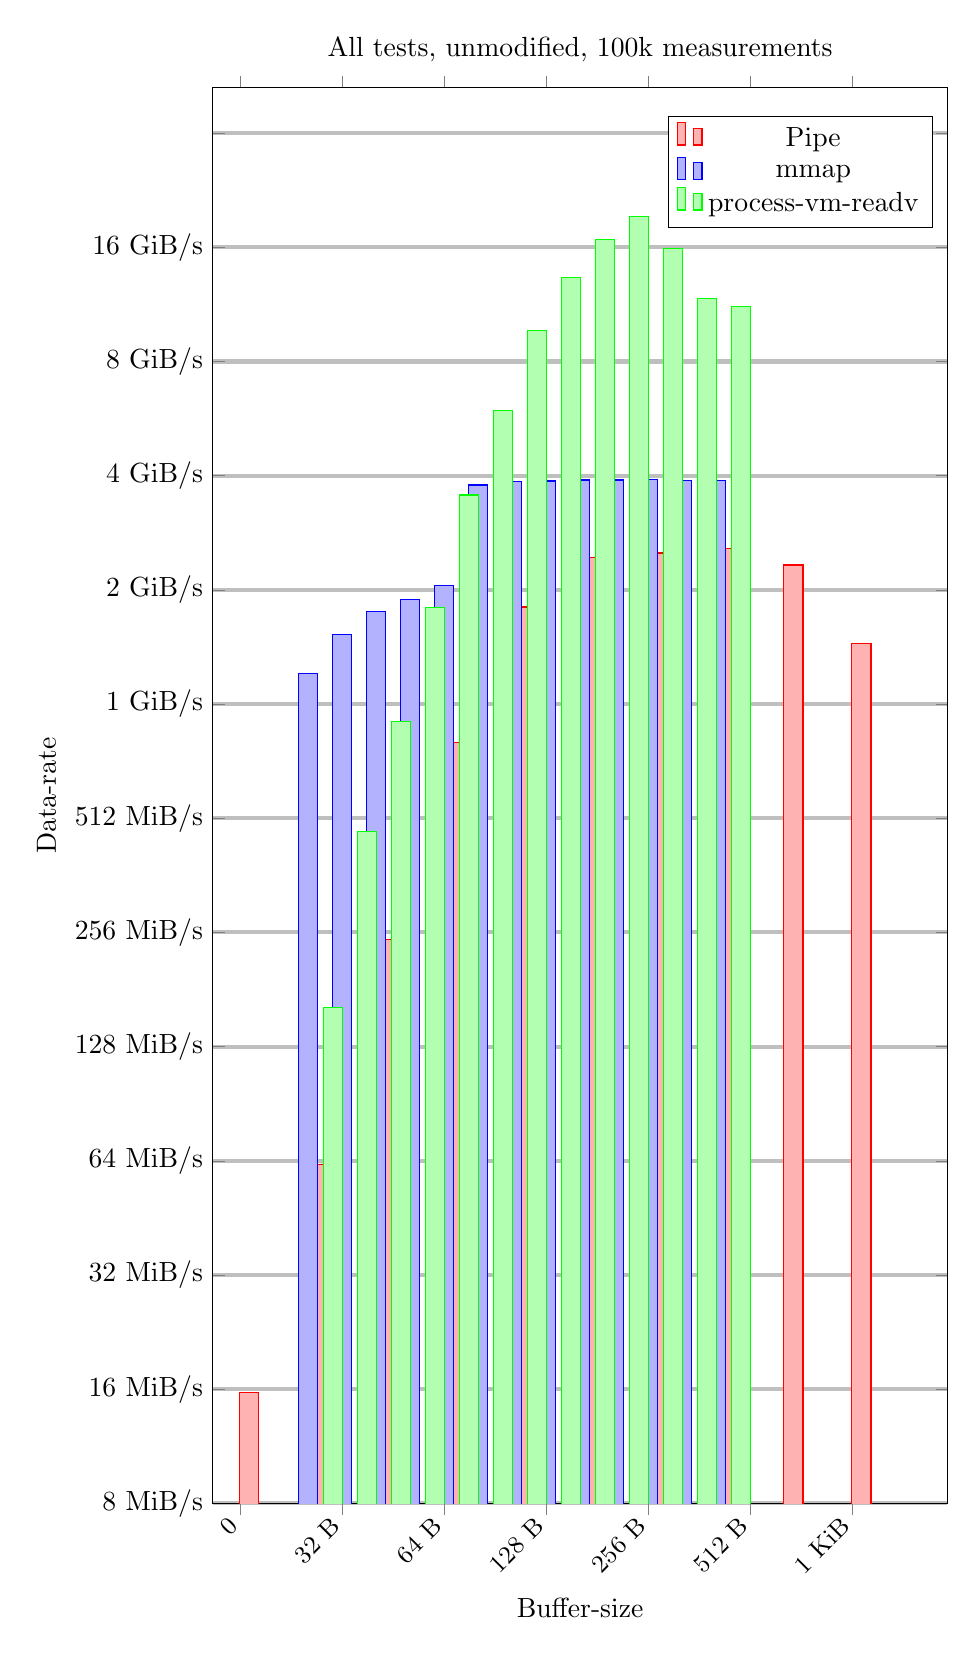
\begin{tikzpicture}
        \begin{axis}[
                ybar,
                xmode=log,
                ymode=log,
                log basis x={2},
                log basis y={2},
                width=0.9\linewidth,
                height=0.7\pdfpageheight,
                xlabel=Buffer-size,
                ylabel=Data-rate,
                xticklabels={0, 32 B, 64 B, 128 B, 256 B, 512 B, 1 KiB, 2 KiB, 4 KiB, 8 KiB, 16 KiB, 32 KiB, 64 KiB, 128 KiB, 265 KiB, 512 KiB, 1 MiB, 2 MiB, 4 MiB, 8 MiB, 16 MiB},
                yticklabels={8 MiB/s, 16 MiB/s, 32 MiB/s, 64 MiB/s, 128 MiB/s, 256 MiB/s, 512 MiB/s, 1 GiB/s, 2 GiB/s, 4 GiB/s, 8 GiB/s, 16 GiB/s},
                x tick label style={rotate=45, anchor=east, font=\small},
                ymin=8,
                ymajorgrids=true,
                major grid style={line width=1.5pt},
                bar width=7pt,
                title={All tests, unmodified, 100k measurements}
            ]

            \addplot[red, fill=red!30] coordinates {
                    (64, 15.68) (256, 62.47) (1024, 244.91) (4096, 809.71) (16384, 1843.20) (65536, 2490.99)
                    (262144, 2558.85) (1048576, 2634.28) (4194304, 2378.18) (16777216, 1479.20)
                };
            \addplot[blue, fill=blue!30] coordinates {
                    (128, 1229.56) (256, 1564.40) (512, 1792.06) (1024, 1932.68) (2048, 2104.00) (4096, 3865.66)
                    (8192, 3956.62) (16384, 3961.44) (32768, 3984.97) (65536, 3985.81) (131072, 3988.44) (262144, 3983.26) (524288, 3979.08)
                };
            \addplot[green, fill=green!30] coordinates {
                    (128, 162.23) (256, 471.83) (512, 918.63) (1024, 1833.78) (2048, 3639.14) (4096, 6060.43)
                    (8192, 9863.89) (16384, 13640.09) (32768, 17125.45) (65536, 19718.39) (131072, 16258.47) (262144, 11989.27) (524288, 11449.94)
                };
            \legend{Pipe, mmap, process-vm-readv}
        \end{axis}
    \end{tikzpicture}
\end{landscape}
\begin{landscape}
    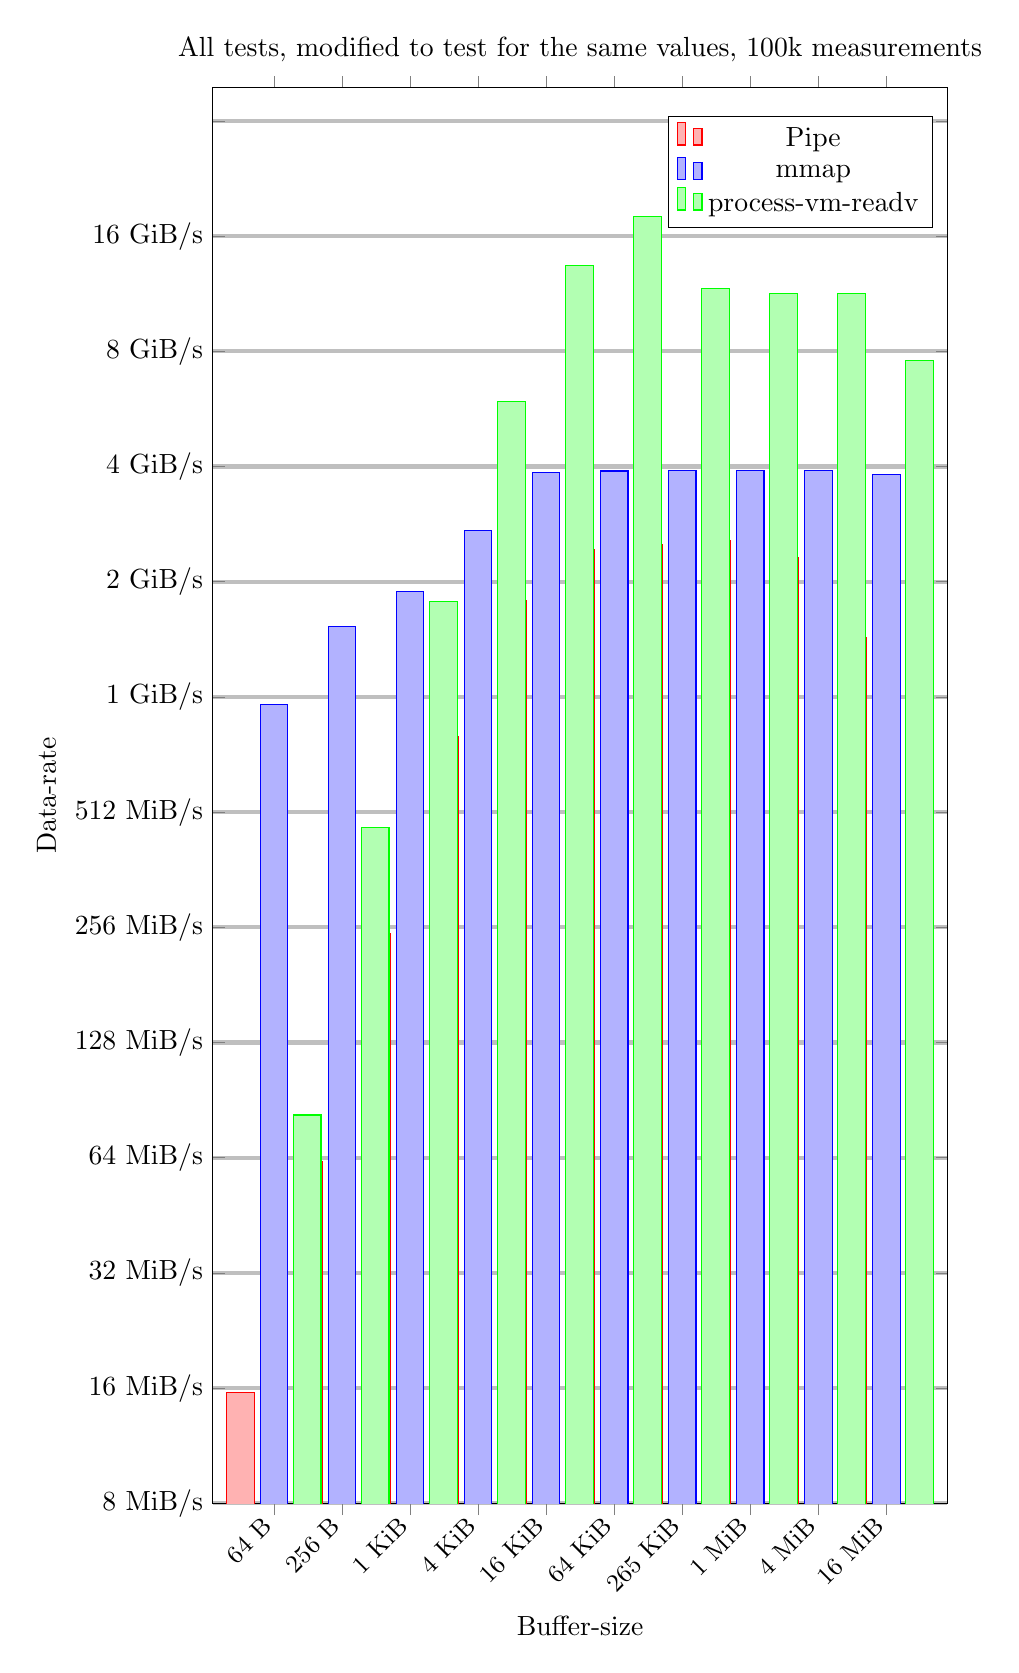
\begin{tikzpicture}
        \begin{axis}[
                ybar,
                xmode=log,
                ymode=log,
                log basis x={4},
                log basis y={2},
                width=0.9\linewidth,
                height=0.7\pdfpageheight,
                xlabel=Buffer-size,
                ylabel=Data-rate,
                xticklabels={0, 64 B, 256 B, 1 KiB, 4 KiB, 16 KiB, 64 KiB, 265 KiB, 1 MiB, 4 MiB, 16 MiB},
                yticklabels={8 MiB/s, 16 MiB/s, 32 MiB/s, 64 MiB/s, 128 MiB/s, 256 MiB/s, 512 MiB/s, 1 GiB/s, 2 GiB/s, 4 GiB/s, 8 GiB/s, 16 GiB/s},
                x tick label style={rotate=45, anchor=east, font=\small},
                ymin=8,
                ymajorgrids=true,
                major grid style={line width=1.5pt},
                title={All tests, modified to test for the same values, 100k measurements}
            ]

            \addplot[red, fill=red!30] coordinates {
                    (64, 15.57) (256, 62.47) (1024, 246.04) (4096, 806.20) (16384, 1828.36) (65536, 2488.33)
                    (262144, 2558.83) (1048576, 2623.03) (4194304, 2363.91) (16777216, 1464.39)
                };
            \addplot[blue, fill=blue!30] coordinates {
                    (64, 977.81) (256, 1564.40) (1024, 1930.88) (4096, 2784.67) (16384, 3940.07) (65536, 3983.27)
                    (262144, 3990.21) (1048576, 3990.46) (4194304, 3985.33) (16777216, 3903.26)
                };
            \addplot[green, fill=green!30] coordinates {
                    (64, 82.74) (256, 466.91) (1024, 1813.79) (4096, 6043.83) (16384, 13709.87) (65536, 18404.44)
                    (262144, 11938.17) (1048576, 11608.91) (4194304, 11562.28) (16777216, 7735.35)
                };
            \legend{Pipe, mmap, process-vm-readv}
        \end{axis}
    \end{tikzpicture}
\end{landscape}
\end{document}